\chapter{Relevant Experiments}\label{chapter:experiments}
    In this chapter, we perform experiments on equations with manufactured solutions using the \textit{NeuroDiffEq} library \citep{chen2020neurodiffeq}, which provides convenient tools for training PINNs. 

    First, we train networks to solve equations and collect their residual information $r$.
    Then, we apply Alg. \ref{alg:single-linear-ode-constant-coeff-loose}--\ref{alg:sde} (where applicable) to derive error bounds using only residual information $r$ and equation structure, characterized by its differential operator $\mathcal {D}$. 
    Lastly, we show that the absolute error strictly falls within the bounds, regardless of how well the networks are trained.

    Throughout this chapter, we always use networks with two hidden layers, each consisting of 32 hidden units.
    Depending on whether the problem is an ODE or PDE, a network can have a single input $t$ or two inputs $(x, y)$, but always have a single output.
    The activation function is $\tanh$. 
    Unless otherwise noted, the training domain is $I=[0, 1]$ for ODEs and $\Omega=[-1,1]^2$ for PDEs. 
    We use a \textit{PyTorch} Adam optimizer with default hyperparameters to train networks for 1000 epochs.

    Notice that we list these configurations only for the reproducibility of visualizations. 
    Our error-bounding algorithm works under any other configurations.

\section{Single Linear ODE With Constant Coefficients}
    Here, we study three equations $v'' + 3v' + 2v = f(t)$, $v'' + v = g(t)$, and $v'' - v' = h(t)$, whose characteristic roots are $\{-1, -2\}$, $\{\pm i\}$, and $\{0, 1\}$ respectively. 
    By Section \ref{section:single-linear-ode-with-constant-coefficients}, the first two equations can be bounded with either Alg. \ref{alg:single-linear-ode-constant-coeff-loose} or Alg. \ref{alg:single-linear-ode-constant-coeff-tight}, while the last must be bounded with Alg. \ref{alg:single-linear-ode-constant-coeff-tight}.

    They all satisfy initial conditions $v(0) = v'(0) = 1$. 
    We pick $f(t) =2t^2+8t+7$, $g(t) = t^2+t+3$, and $h(t)=1-2t$, so that the manufactured solution is $v(t) = t^2 + t + 1$ for all three equations.
    Fig. \ref{fig:2nd-order-bound} shows that both $\Bound_{loose}$ (Alg. \ref{alg:single-linear-ode-constant-coeff-loose}) and $\Bound_{tight}$ (Alg. \ref{alg:single-linear-ode-constant-coeff-tight}) strictly bounds the absolute error.
    
    \begin{figure}[!ht]
        \centering
        \includegraphics[width=\linewidth]{assets/2nd-order.pdf}
        \caption{
            Loose bound (Alg. \ref{alg:single-linear-ode-constant-coeff-loose}) and tight bound (Alg. \ref{alg:single-linear-ode-constant-coeff-tight}) for 3 second-order linear ODE with constant coefficients.
            Notice that the loose bound cannot be applied to the third equation since it has characteristic roots with positive real part.
        }\label{fig:2nd-order-bound} 
    \end{figure}

\section{Linear ODE System with Constant Coefficients} \label{section:high-dimension}
    In this section, we train $6$ networks to solve a $6$-dimensional linear system of ODEs with constant coefficients, namely, $\frac{\mathrm{d}}{\mathrm{d}t}\vect{v} + A\vect{v} = \vect{f}$. 
    We pick $A = PJP^{-1}$ where {$J=\begin{pmatrix}J_1\\[-1.25ex]&J_2\\[-1.25ex]&&J_3\end{pmatrix}$} with {$J_1 = \begin{pmatrix} 4&1\\[-1.25ex]&4&1\\[-1.25ex]&&4\\[-0.5ex]\end{pmatrix}$, $J_2 = \begin{pmatrix} 3&1\\[-1.25ex]&3\\[-0.25ex]\end{pmatrix}$ }, $J_3=2$, and $P$ is a random orthogonal matrix.

    We pick the initial conditions to be {$\vect{v}(0) = P(0\, 0\, 1\, 0\, 1\, 1)^{T}$} and the forcing function to be {$\vect{f}(t) = P(\cos t + 4 \sin t  + \ln(1+t),\, \frac{1}{1+t} + 4 \ln(1+t) + (t+1),\, 4t + 5,\, 2t + 3t^2 + e^t,\, 4 e^t,\, 2 \cos t - \sin t )^T$}, so that the manufactured exact solution is {$\vect{v}(t) = P ( \sin t,\, \ln(t + 1),\, t + 1,\, t^2,\, e^t,\, \cos t)^T$}.

    After obtaining the residual information {$\vect{r}(t)=\frac{\mathrm d}{\mathrm d t}\vect{u}(t) + A\vect{u}(t) - \vect{f}(t)$}, we apply Alg. \ref{alg:system-bound} to obtain componentwise bound and norm bound of {$\pmb{\Err} = \vect{u}-\vect{v}$}. 
    It is shown in Fig. \ref{fig:system-bound} that the bounds hold over the domain.

    \begin{figure}[!ht]
        \centering
        \includegraphics[width=\linewidth]{assets/system-bound.pdf}
        \caption{\textit{Componentwise} bound (upper) and \textit{norm} bound (lower) for linear ODE system with constant coefficients}\label{fig:system-bound}
    \end{figure}

\section{Nonlinear ODE -- Duffing Equation} \label{section:experiment-duffing}
    In this section, we consider a Duffing oscillator, which is characterized by the following $2$nd order nonlinear ODE:
    {
        \begin{equation}\label{eq:duffing}
            \frac{\mathrm{d}^2 v}{\mathrm{d}t^2} + 3 \frac{\mathrm{d}v}{\mathrm{d}t} + 2v +\varepsilon v^3 = \cos t ,
        \end{equation}
    }
    under initial conditions $v(0) = 1$ and $v'(0) = 1$, where $\varepsilon$ controls the nonlinearity of the equation. 
    Using Alg. \ref{alg:nonlinear-iterative}, we solve the equation on $I=[0, 2]$ for linspaced $\varepsilon \in (-0.9, 0.9)$ using neural networks and bound the errors. 
    The input $J$ to Alg. \ref{alg:nonlinear-iterative} is chosen to be $6$. 
    Namely, we expand the solution and bound components from degree $0$ to $6$.

    The analytical solution to Eq. \eqref{eq:duffing} is complicated. 
    Hence, we use the RKF4(5) method to compute numerical solutions that are close enough to exact solutions for visualization purposes. 
    See Fig. \ref{fig:duffing-solution} for network solutions against RKF4(5) solutions and Fig. \ref{fig:duffing-error} for error bounds against absolute error.
    \begin{figure}[!ht]
        \centering
        \includegraphics[width=\linewidth]{assets/duffing-solution.pdf}
        \caption{RKF45 and Network Solutions (max-degree 0$\sim$6) to Duffing equation \eqref{eq:duffing} for $\varepsilon \in (-0.9, 0.9)$}\label{fig:duffing-solution}
    \end{figure}
    \begin{figure}[!ht]
        \centering
        \includegraphics[width=\linewidth]{assets/duffing-error.pdf}
        \caption{True Error vs. error bound (max-degree 0$\sim$6) of neural network solution to Duffing Equation \eqref{eq:duffing} for $\varepsilon \in (-0.9, 0.9)$}\label{fig:duffing-error}
    \end{figure}

\section{Linear PDE System with Nonconstant Coefficients } \label{section:experiment-attractor}
    \begin{figure}[!ht]
        \centering
        \subfloat[\centering $\mathcal{C}: \begin{cases*} x' = -x - y \\ y' = x - y \end{cases*}$]{{\includegraphics[width=0.50\linewidth]{assets/characteristics.pdf}}}
        \subfloat[\centering $\mathcal{C}: \begin{cases*} x' = x^2 + y^2 + 1 \\ y' = x^2 - y^2 + 2 \end{cases*}$]{{\includegraphics[width=0.49\linewidth]{assets/unsolvable-characteristics.pdf}}}
        \caption{
            Characteristics curves of Eq. \eqref{eq:attractor} (left) and Eq. \eqref{eq:hard-to-solve-characteristics} (right). 
            The red curves, with staring points $A$ to $P$, are selected for visualization of absolute error and error bound in Fig. \ref{fig:pde-error-bound}.
        }\label{fig:characteristics}
    \end{figure}

\subsection{PDE Error Bound Evaluation Using Alg. \ref{alg:linear-first-order-pde-general}}
    \begin{figure}[!ht]
        \centering
        \includegraphics[width=\linewidth]{assets/pde-error-bound.pdf}
        \caption{
            Absolute error and error bound on selected characteristic curves. 
            These characteristic curve start at points $A$ through $P$ as shown in Fig. \ref{fig:characteristics}a.
            The blue solid curves are absolute error along the characteristic curves and red dotted curves are corresponding bounds.
        }\label{fig:pde-error-bound}
    \end{figure}

    We try to solve the following first-order linear PDE,
    {
        \begin{equation} \label{eq:attractor}
            (-x -y) \px{v} + (x - y) \py{v} + v = 3x - 2 y
        \end{equation}
    }
    in spatial domain $\Omega=[-1, 1]^2$. 
    The boundary constraints are $v(x, \pm1) =2x\pm 3$ and $v(\pm 1, y) = 3y \pm 2$. 
    The manufactured solution is given by $v(x, y) = 2x + 3y$.
    The characteristic curves are integral curves {$\mathcal{C}: \begin{cases*} x'(s) = -x - y \\[-0.25em] y'(s) = x - y \end{cases*}$}, or {$\mathcal{C}:\begin{cases*} x(s) = R_0 e^{-s} \cos (s+\theta_0)\\[-0.25em] y(s) = R_0 e^{-s} \sin(s + \theta_0) \end{cases*}$}, where $R_0 = \sqrt{x_0^2+y_0^2}$ and $\theta_0 = \mathrm{atan2}(y_0, x_0)$ are constants determined by the starting point $(x_0, y_0) \in \Gamma = \partial \Omega$.
    See Figure \ref{fig:characteristics} for visualization.

    Since the analytical expression of the characteristic curves is known, Alg. \ref{alg:linear-first-order-pde-general} can be applied to evaluate the bound on each curve. 
    We choose $16$ characteristic curves with starting points $A$, $B$, \dots, $P$, equidistantly placed on the boundary (Fig. \ref{fig:characteristics}a). 
    We plot the absolute error and the computed error bound along these characteristic curves in Fig. \ref{fig:pde-error-bound}.
    It can be seen that absolute error lies strictly within the bounds.
\subsection{PDE Error Bound Evaluation Using Alg. \ref{alg:linear-first-order-pde-constant}}
    Consider the following PDE 
    {
        \begin{equation}\label{eq:hard-to-solve-characteristics}
            (x^2+y^2+1)\px{v} + (x^2-y^2+2)\py{v} + (3-2x)v = f
        \end{equation}
    }
    over domain $\Omega = [-1, 1]^2$, where $f(x, y) = 6-4x$.
    The boundary constraints are $v(-1, y) = 2$ and $v(x, 1) = 2$ and the manufactured solution is $v(x, y) = 2$.
    
    The characteristic curves {$\mathcal{C}: \begin{cases*} x'(s) = x^2+y^2+1 \\[-0.25em] y'(s) = x^2 - y^2 + 2 \end{cases*}$} are given by a nonlinear ODE, which is hard to solve analytically. 
    (See Fig. \ref{fig:characteristics}b for visualization)
    Therefore, Alg. \ref{alg:linear-first-order-pde-general} cannot be applied to evaluate the error bound. 

    However, the coefficient $(3-2x)$ is nonzero over domain $\Omega$.
    Hence, we can use Alg. \ref{alg:linear-first-order-pde-constant} to compute a constant error bound $|\eta(x, y)| \leq \Bound(x, y) \equiv B$ for all $(x, y) \in \Omega$.
    We visualize the bound and the maximum absolute error $\max_{(x, y)\in\Omega}|\Err|$ after each training epoch in Fig. \ref{fig:pde-constant-bound}.
    As expected, the bound is loose, which is about an order of magnitude larger than the max absolute error.
    Yet, it consistently holds true for every epoch, even during the early stages of training, when the network performs poorly.
    \begin{figure}[!ht]
        \centering
        \includegraphics[width=\linewidth]{assets/pde-constant-bound.pdf}
        \caption{
            Constant bound $B$, computed using Alg. \ref{alg:linear-first-order-pde-constant}, and max absolute error over domain at different epochs of training.
        }\label{fig:pde-constant-bound}
    \end{figure}

\section{Linear SDE}
    In this section, we verify the validity of error-bounding algorithm \ref{alg:sde} on the following stochastic differential equation:
    \begin{equation}\label{eq:sde-experiment}
        \d V_t = \big(e^{-t} -(2t + \sin t) V_t \big)\d t + \ln(t+5) \d W_t
    \end{equation}
    We compute 10 true error paths by taking the difference between the network solution $u(t)$ and 10 different realizations $V_t$, which are computed using stochastic Runge-Kutta method proposed by \citeauthor{rossler2010runge} \cite{rossler2010runge} for strong apprxoimation of SDEs.

    We verify that the error bound $|\Eta_t| \leq \Bound_{\epsilon}(t) = \Bound'_{\frac{\epsilon}{2}, \frac{\epsilon}{2}}(t)$, where $\Bound'_{\epsilon_1, \epsilon_2}$ is defined by Eq. \eqref{eq:bound-two-epsilon}, holds with at least desired probability $(1-\epsilon)$ for $\epsilon \in \left\{ 0.1, 0.2, \dots, 0.6\right\}$.
    As shown in Fig. \ref{fig:sde-bound-1}.

    \begin{figure}[!ht]
        \centering
        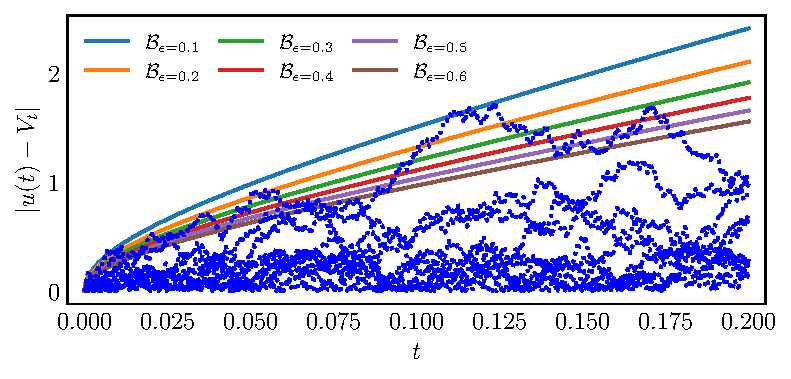
\includegraphics[width=\linewidth]{assets/sde1.pdf}
        \caption{
            Error and error bound for stochastic differential equation \eqref{eq:sde-experiment}. 
            Solid lines are error bounds $\Bound_{\epsilon}$ that hold with probability at least $1-\epsilon$ for $\epsilon = 0.1,\, 0.2,\, \dots,\, 0.6$ and dotted lines are error paths from 10 different realizations. 
        }\label{fig:sde-bound-1}
    \end{figure}